\documentclass[11pt]{article}

%\usepackage{amsmath, amssymb, fullpage, amsthm, array, algorithm2e,graphicx}
\usepackage{graphicx}
\usepackage{url}
\RequirePackage{natbib}
\usepackage[colorlinks=true, citecolor=blue, linkcolor=blue]{hyperref}

\graphicspath{{images/}}

\setlength{\oddsidemargin}{0in}
\setlength{\evensidemargin}{0in}
\setlength{\textwidth}{6.5in}
\setlength{\topmargin}{-0.3in}
\setlength{\textheight}{8.8in}


%\setlength{\evensidemargin}{0.25 in}
%\setlength{\textwidth}{6.2 in}           % allow for a little sloppiness (6.3)
%\setlength{\topmargin}{-.30 in}           % top margin to header (was -.35)
%\setlength{\textheight}{8.8 in} 


\title{Designing Turk Experiments for Visual Statistical Inference}
\author{Mahbubul Majumder, Heike Hofmann, Dianne Cook\\
        Department of Statistics, Iowa State University}


\begin{document}

\tableofcontents

\maketitle


\begin {abstract} 

Human observers are needed to evaluate lineups that are used to test the significance of findings using statistical graphics. One good option is to recruit people from online workplace like Amazon Mechanical Turk (MTurk). It has the facilities to create online task that would allow people to evaluate lineups and get paid. MTurk is designed for simple and easy tasks. The technical design of the underlying experiment for visual inference may be complex and the tools available to design this from MTurk is just too simple. In this paper we describe how to design MTurk experiments, present an alternative way to conduct the survey on lineups by designing a separate web application and getting turk worker do their job from this web site. The web site is now hosted on the Iowa State University public domain and has been in use for multiple experiments \citep{majumder:turk}. It turns out to be a very efficient way of getting lineups evaluated by online observers. Getting results from this web site is very convenient and secure.

\end {abstract}


\section{Introduction} 

There have been some advancements in visual statistical inference since it was first introduced by Buja \cite{buja:2009} where they have proposed formal methods for testing the significance of findings using lineup protocols. In visual statistical inference the test statistics is a plot of the observed data. This plot is placed randomly in a layout of plots called lineup. The rest of the plots in the lineups are generated from the model specified by the null hypothesis. A human observer is asked to evaluate the lineup. If the observer detects the actual plot in the lineup, the null hypothesis is rejected. 

A lineup is shown in Figure~\ref{fig:lineup_turk} where the observed scatterplot is displayed with a least square line overlaid. Can you find which of these plots show the steepest slope? The rest of the plots or the null plots are generated based on the hypothesis that the slope is zero. If the observed scatterplot is detected that indicates that observed plot is different from null plot and hence the null hypothesis is rejected.

\begin{figure}[htbp] 
   \centering
   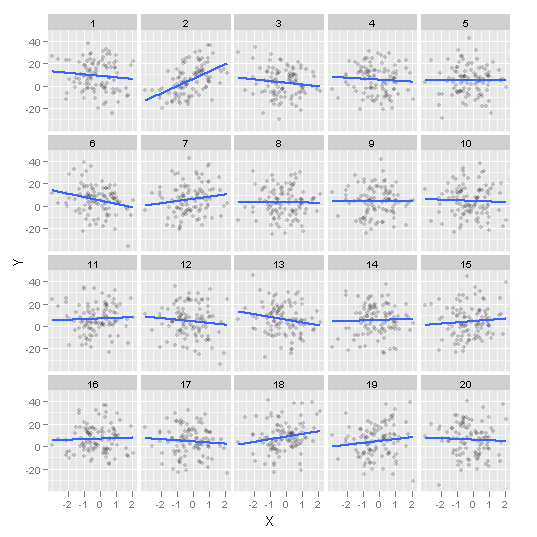
\includegraphics[width=6.5in]{plot_turk2_100_450_12_3.png} 
   \caption{A lineup of 20 scatter plots with least square line overlaid. Which of these plots shows the steepest slope?.}
   \label{fig:lineup_turk}
\end{figure}


The power of visual test is studied by \cite{majumder:2013} and it is revealed that power could be as good as conventional test and in some scenerios even better. But where the conventional test does not exists, visual inference could be the only inferential procedure without compromising a lot in power. 

These developments open up a whole new area of statistical research where lineups need to be evaluated by human observer. There are some reasons a researcher needs to evaluate lineups. One is to assess the power of the visual test \citep{heike:2012} for different visual test statistics. The another reason would be to make decision based on the lineup, i.e., to use lineup protocol in practical application \citep{niladri:2012}. Other reasons could be to present the results of the conventional test with visual tools such as lineup.  



%The effect of different graphical design while selecting visual test statistic is studied by Heike \cite{heike:2012}.

The power of visual test can be obtained theoretically under some assumptions on individual behavior which was evident from experimental studies \citep{majumder:2013}. In general it is hard to obtain explicitly with a mathematical formula since it is very much dependent on individual observation. One approach to estimate the power is to recruit observers to evaluate lineups obtained in known controlled situation. Individual differences in the abilities of correct evaluations of lineup were observed. But Observer's education levels do not seem to have significant effect on performances. Thus it is better to get observers as diverse as possible without being much concerned about the observers' formal training about statistical graphics.

This poses a new challenge to researcher to recruit people from a diverse pool of population. Cost, time, data qualities and convenience are some of the issues that need to be dealt with. Fortunately, we can use the services of Amazon Mechanical Turk web site for this.  

\subsection{Amazon Mechanical Turk (MTurk)}

\cite{turk} Mechanical Turk  or MTurk is an online work place where people from around the world can perform some tasks and get paid. Usually tasks are very simple and no specialized training is required. Being a human is the main requirement. Tasks are designed for anyone to do but some tasks may require that workers satisfy some skill level depending on the recruiters' need. The tasks are designed such that it does not take much time to complete. Humans are still better than computers in performing these types of tasks. The the amount of money paid for each task is very small as well. Figure~\ref{fig:amazon_task} shows an MTurk task where an observer is asked to select from some given options based on a picture. 


\begin{figure}[htbp] 
   \centering
   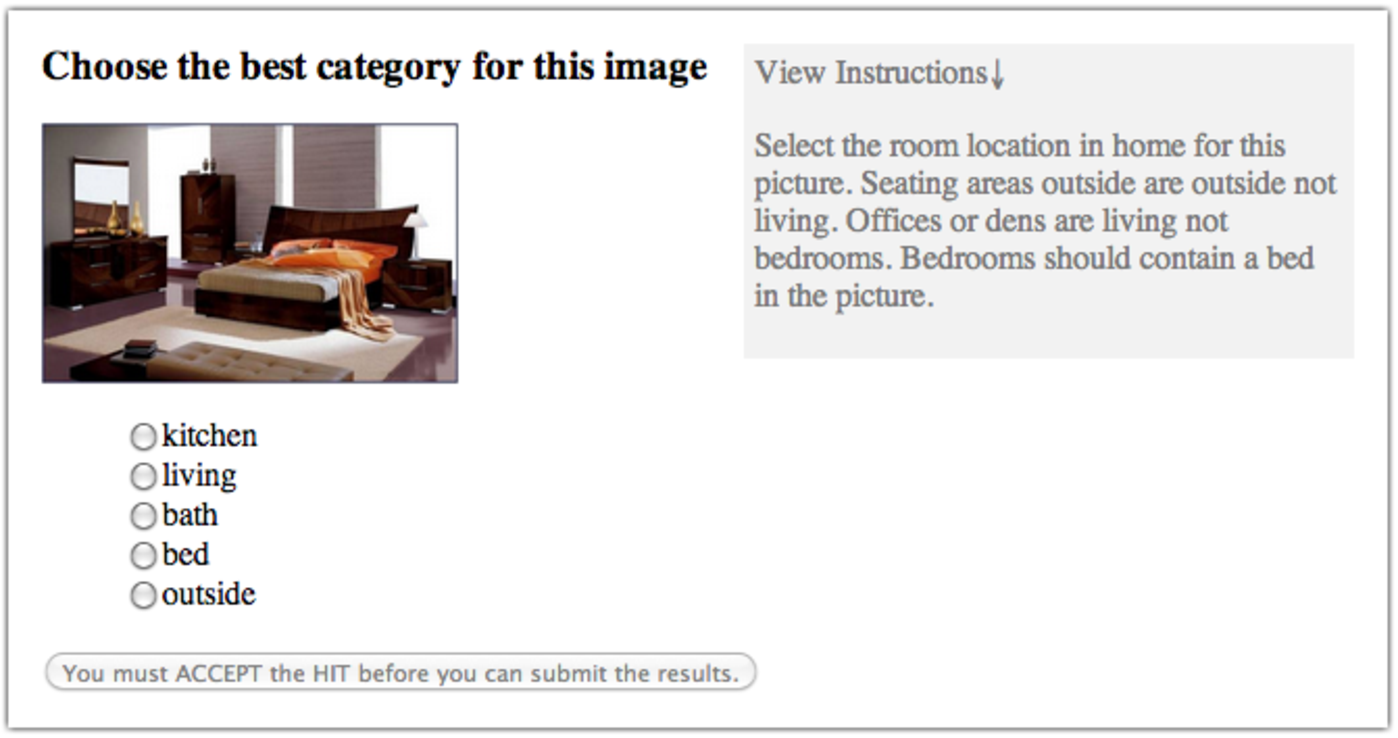
\includegraphics[width=5in]{amazon_task.pdf} 
   \caption{An example of amazon mechanical turk task. Tasks are usually very simple and designed for human evaluations. With each task, simple instructions are given for workers to follow. The workers first accept the task before submitting their response.}
   \label{fig:amazon_task}
\end{figure}



It is very fast, cheap and reliable to recruit people from MTurk. It allows distributing works to the thousands of workers around the world. Thats why it is getting very popular among the researchers who perform human subject experiment. The another benefit is that a very diverse pool of subjects can be recruited which is otherwise very hard to obtain for a study. The researchers can easily filter the workers based on their experimental design, such as recruiting people only from a specific geographical location or a group of people who satisfy certain criteria etc. The recruiter can decide who they pay or not. Workers have to satisfy the task requirement to ensure payment. But at the end it is the recruiter who has the final say. Usually recruiters pay promptly after the task has been done properly and thats why MTurk is very popular among the online job seeker. 

Because of its convenience it is getting popular for scientific research study as well. In comparison with a lab study \cite{suri:2010} performed the same study using MTurk and demonstrated that their study results are as good as the lab study results even though MTurk study required less time and cost while provided more convenience. \cite{majumder:2013} recruited people from MTurk for their simulation study in estimating the power of visual statistical inference. They have done numerous pilot studies in lab before doing actual MTurk study and found similar results. \cite{mason:2012} explains various features of MTurk and describes how it can be used as part of human behavioral study.

Figure \ref{fig:amazon_task} shows how simple an MTurk task could be. It is possible to get a lineup evaluated by creating such a simple task. We just need to replace the picture in Figure \ref{fig:amazon_task} with the lineup in Figure \ref{fig:lineup_turk} and change the answering options. But some times we may need more than one lineups to be evaluated by an observer. We may need to show a random sample of lineups from a pool of many lineups automatically. The questions the observer would answer while examining the lineup can be different based on different lineup. Moreover, It is convenient if the lineup is clickable so that selection of plot can be made by mouse click. All these are done by creating a web application. The following section discusses this in details.



%Amazon Mechanical Turk web site \cite{turk} is a very good resource for recruiting reliable survey participants for visual experiments. This is the place where people come to work online and get paid. The web site is very convenient and reliable to collect simple experiment data. But to design a complex experiment like what we need using their web interface is a pain and often a very time consuming work. So, to run the turk experiment we felt the necessity for a well customized web site where the lineups presented to the observers could be easily controlled according to the experimental design. The work flow design of such a mechanism is shown in figure \ref{fig:turk_work_flow}. The plan is to forward turk workers to a well customized web site while payment could be processed from turk web site. This facilitates getting data directly in a local server.

%Figure \ref{fig:amazon_task} displays an example of such a task taken from their web site. In this task a worker just has to select from a pool of options and submit the task. The instructions are usually accompany the task and they are very simple and easy to follow. 

\subsection{Getting Turk Workforce}

There are two options to run the web application; one is to run it inside MTurk system using their API and the other is to develop a new web site. For additional control we picked the second option and planned to separate this application from MTurk system and designed our own web site to run the application. It enables to display the lineups to the observers with a lot of flexibilities. As an added benefit the data can be directly saved in a local database server instead of getting it from MTurk. 

Figure \ref{fig:turk_work_flow} shows how the plan works. First an MTurk task is created for the workers to see and decide whether they want to do the task based on the parameters like payment amount, estimated time the task may take to finish, how hard the task seems to be etc. Workers are informed that the task has to be done outside the MTurk system from another web site. Once the workers accept the task they are redirected to our web site where multiple lineups are shown for evaluations. After the required number of evaluations has been received, a code is generated which the workers has to submit back in MTurk system to complete the task. The code is matched with the code in our database to process payment through MTurk system.

\begin{figure}[htbp]
   \centering
       \scalebox{.4}{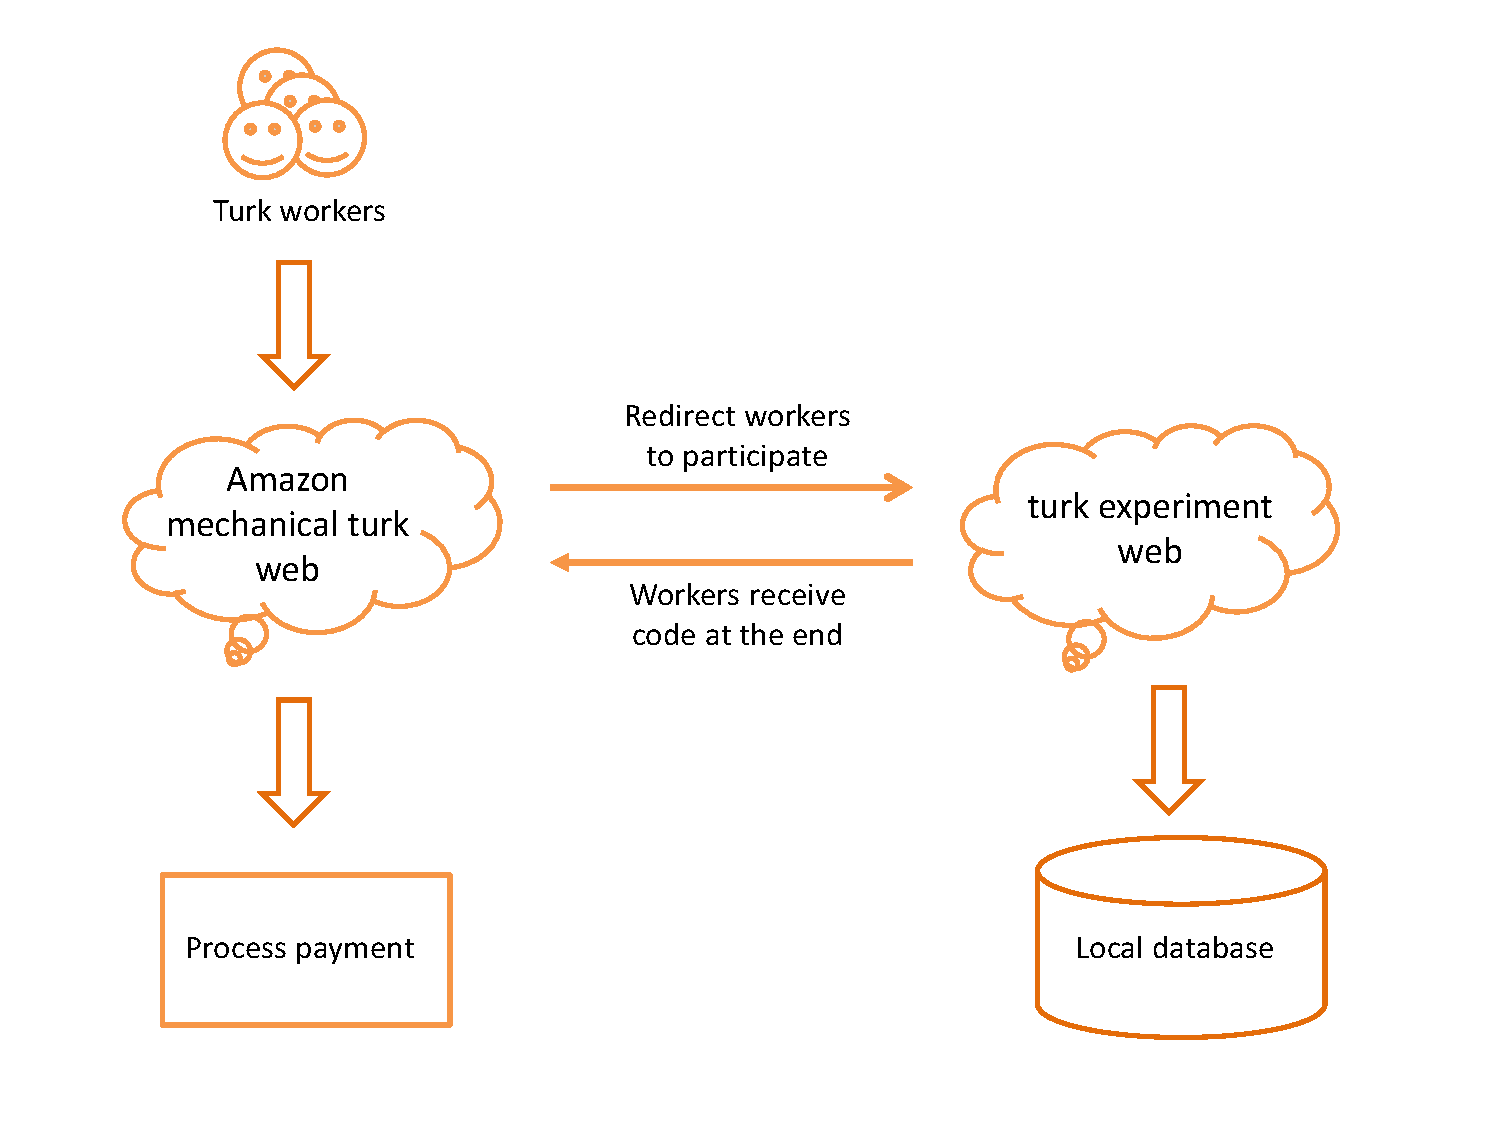
\includegraphics{turk_work_flow.pdf}}
       \caption{Amazon Mechanical Turk workflow shows how data are collected through turk experiment web and payment is processed through MTurk system.}
       \label{fig:turk_work_flow}
\end{figure}

MTurk will provide workers who are used to doing simple task. Thus, for lineups to be evaluated a simple task needs to be created through MTurk. But People who need to make statistical decision based on lineup will need a system that can provide an easy solution to this challenge.  This paper provides a complete solution to this. This paper is organized the way a researcher may work with lineup and like to get feedback data from the observer. Section \ref{sec:turk_exp} presents the details description of an experiment with lineups and things to consider before a turk task. Section \ref{sec:web_application} presents the design of an web application to get lineups evaluated with additional flexibilities and options that may not possible through MTurk. Section \ref{sec:turk_task} describes how to create an MTurk task, mange workers and process payments. Finally Section \ref{sec:turk_data} presents some data obtained from various experiments done through the web application and discusses about the quality of the data.


\section{Experiment Design} \label{sec:turk_exp}

If a lineup is already created from observed data, the web application presented in Section \ref{sec:web_application} can be used to evaluate it. In this scenario we do not need to design an experiment. This section will be useful when a simulation experiment is needed to examine different plot types as test statistics and compare the power of visual test \citep{majumder:2013}. To examine the effectiveness of certain plots in displaying the data one might want to design an experiment with lineup \citep{heike:2012}. In any cases, two major considerations are choice of parameters to simulate lineup and number of people needed to be recruited to evaluate a lineup.

\subsection{Selecting Parameter to Simulate Lineup} The first consideration for a simulation experiment is to fix the parameters of the model of interest. The very first consideration is the sample size. Other parameters depends on the model of interest. For example we have fixed the parameters in our first Amazon Mechanical Turk experiment as shown in table \ref{tbl:experiment_params}.

\subsection{Procedure to Simulate Data Plot} \label{sec:simulate_plot} In the simulation study the very first step is to generate a random sample of data from model of interest for prespecified parameters. We call this data set observed data. While the effect of the natural variability of this data set could be contolled by taking the replication of few samples, it is desirable to study whether we can reduce this variability alternatively. The main reason is to minimize the cost. To make sure that the observed data set truly represents model of interest we are considering three approaches. One is Kolomogorov test statistic approach and the other two approaches are quantiles of p values and closeness of estimated parameters to the true parameters. These three approaches are discussed below.\\

{\bf Kolomogorov test statistic approach:} In this approach we simulate 1000 data sets and obtain Kolmogorov test statistic for each set of data as below. $$D_n=\sup_x |F_n(x)-F(x)|$$ where $F_n(x)=\frac1n \sum_{i=1}^n I_{X_i\le x}$ be the empirical distribution function of fitted residuals, $I_{X_i\le x}$ be the indicator function equal to 1 if $X_i\le x$ and equal to 0 otherwise and $F(x)$ be the cumulative function of normal with mean zero(0) and variance $\sigma^2$. We then keep the data set that has minimum value for Kolmogorov test statistic.  For replication purpose we can generate three observed data sets in similar way.\\

{\bf Quantiles of p-value approach:} With any data set we generate there is a p-value associated with testing $H_0: \beta=0$. In this approach we generate 1000 data sets from the model of interest and obtain p-values associated with $H_0: \beta=0$ for each data set after fitting the same model. Then we construct blocks of p-value such as (0.0-$q_{33}$), ($q_{33}$-$q_{66}$), ($q_{66}$-1) where $q_i$ is the $i$th percentile in the distribution of the p-values. We then randomly select three data sets that have corresponding p-values in the above quantile range. As an example the distribution  of p-values in 1000 simulated data sets for $n$=300, $\beta$=3 and $\sigma$=12 is shown in figure \ref{fig:dist_pvalue}.  Notice that if we like to have three replications of plots, we will have observed data sets with smaller p-values as the distribution is highly right skewed as well as the 33th and 66th percentiles of p-values are 0.0101 and 0.077 respectively. So, another option may be to take the mid points of those quantile ranges and pick the data sets that have those p-values.\\

\begin{figure}[hbtp]
   \centering
       \scalebox{.3}{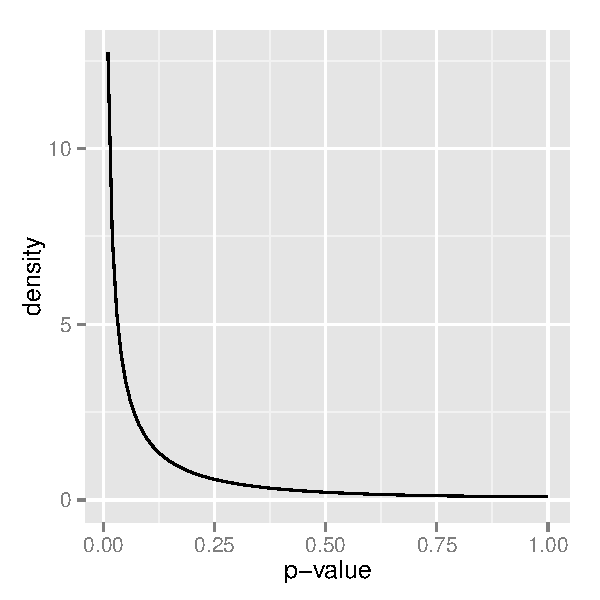
\includegraphics{dist_pvalue.pdf}}
       \caption{Distribution of p-values for $n$=300, $\beta$=3 and $\sigma$=12.}
       \label{fig:dist_pvalue}
\end{figure}

{\bf Closeness of estimated parameters:} When we simulate a data set from the model of interest and again fit the same model with the data set we do not get the parameters estimates same as what we fixed while simulation. It depends on what the standard errors of the parameter estimates are. In our experimental setting we some times have very different estimates for small parameter values(such as one may get estimated value of 0.5 for true $\beta=3$). In this approach we pick the data set that shows most close estimates of parameters compared to true parameter values.\\

All of these three approaches discussed above has some problems. Kolmogorov method does not necessarily make sure that estimated parameters are close to the true parameters. On the other hand closeness of estimated parameters does not make sure that p value is small enough when we should reject the null hypothesis. Only the quantiles approach seems reasonable as it has much control over p-values and it gives similar data sets that has closest parameter estimates. So we used the quantiles of p-value approach in section \ref{sec:simulate_plot} to obtain three replicated sample of observed data sets for a particular parameter settings.\\

\subsection{Sample size estimation} For a given proportion $p$ we want to have margin of error (ME) to be 0.1. Thus we have $$ME =1.96 \sqrt{ \frac 1 n p(1-p)} \le 0.05$$ which gives us the estimation of minimum sample size $$n \geq \frac{p(1-p)}{(0.05/1.96)^2}.$$ Now from the theoretical power curve for each parameter combinations shown in table \ref{tbl:experiment_params} we know the power(say $p$) and thus we can estimate the sample size required for that specific combinations of parameter. We collect data such that each of the parameter combinations in the table \ref{tbl:experiment_params} has approximately the estimated sample size that we calculated here.


\subsection{Test and Training Lineup} How many test lineup?

How to setup training, randomized or sequential selection of lineup for training.

Example lineup on the homepage should be of size three or four so that more than one lineup can be placed on the homepage.

\subsection{Planing the Turk Task}
Question to ask

Whether reasoning would be collected or not

Multiple or single response

Test plot added or not

Training needed or not

Feedback given after every evaluation or not

How many lineups to show

Are the lineups randomly selected?


\section{Web Application for Turk Experiment} \label{sec:web_application}

A web site is developed to get lineups evaluated by human observers \citep{majumder:turk}. It provides all the features needed for a simulation experiment with lineups but yet remains simple for the online workers. This section describes the technical details of the site. 

The web application is built using server side scripting language PHP embedded in HTML. JavaScript is used to control the client side work flow such as preventing missing information, showing messages etc. MySQL database is used to store data for dynamic presentation of lineup and recording observer feedbacks. The application also records the ip address of the observer's machine and the time of each display of lineup and its evaluation.  

%We developed a web site to run the Amazon Mechanical Turk experiments.  PHP scripting language is used and embedded with HTML for designing the web site. Javascript is used for validating the input data and producing warning message.  We use  Amazon Mechanical Turk web site to recruit the participants and direct them to our web site to actually participate in the survey. This has allowed us to get the data directly in a secure way from the web and we don't have to depend on the Mechanical Turk web site to transfer data to our server. 

\subsection{Form Design}

Designing a data collection form is very critical in turk experiments. As we see from Figure \ref{fig:amazon_task} that a turk task needs to be as simple as possible. This is what the turk workers are prepared for. Making a complex form may turn out bad and jeopardize the whole purpose of the experiment. 

Keeping these in mind, two web forms are designed to collect information from the turk workers. The first form shown in Figure \ref{fig:turk_web} collects feedback information about a single lineup. The information collected through this form is all about the lineup that includes plot number selected, reasons for selection and the confidence level of the selection. Each turk user is identified by the nick name which is mainly the turk ID. It looks simple and it is indeed simple for the turk worker to provide feedback using this form. But it is not simple in design as all the information on this form are coming from database including the question on top of the lineup. This dynamic page provides a lot of features in customizing how one may want to display the lineup.

\begin{figure}[hbtp]
   \centering
       \scalebox{.4}{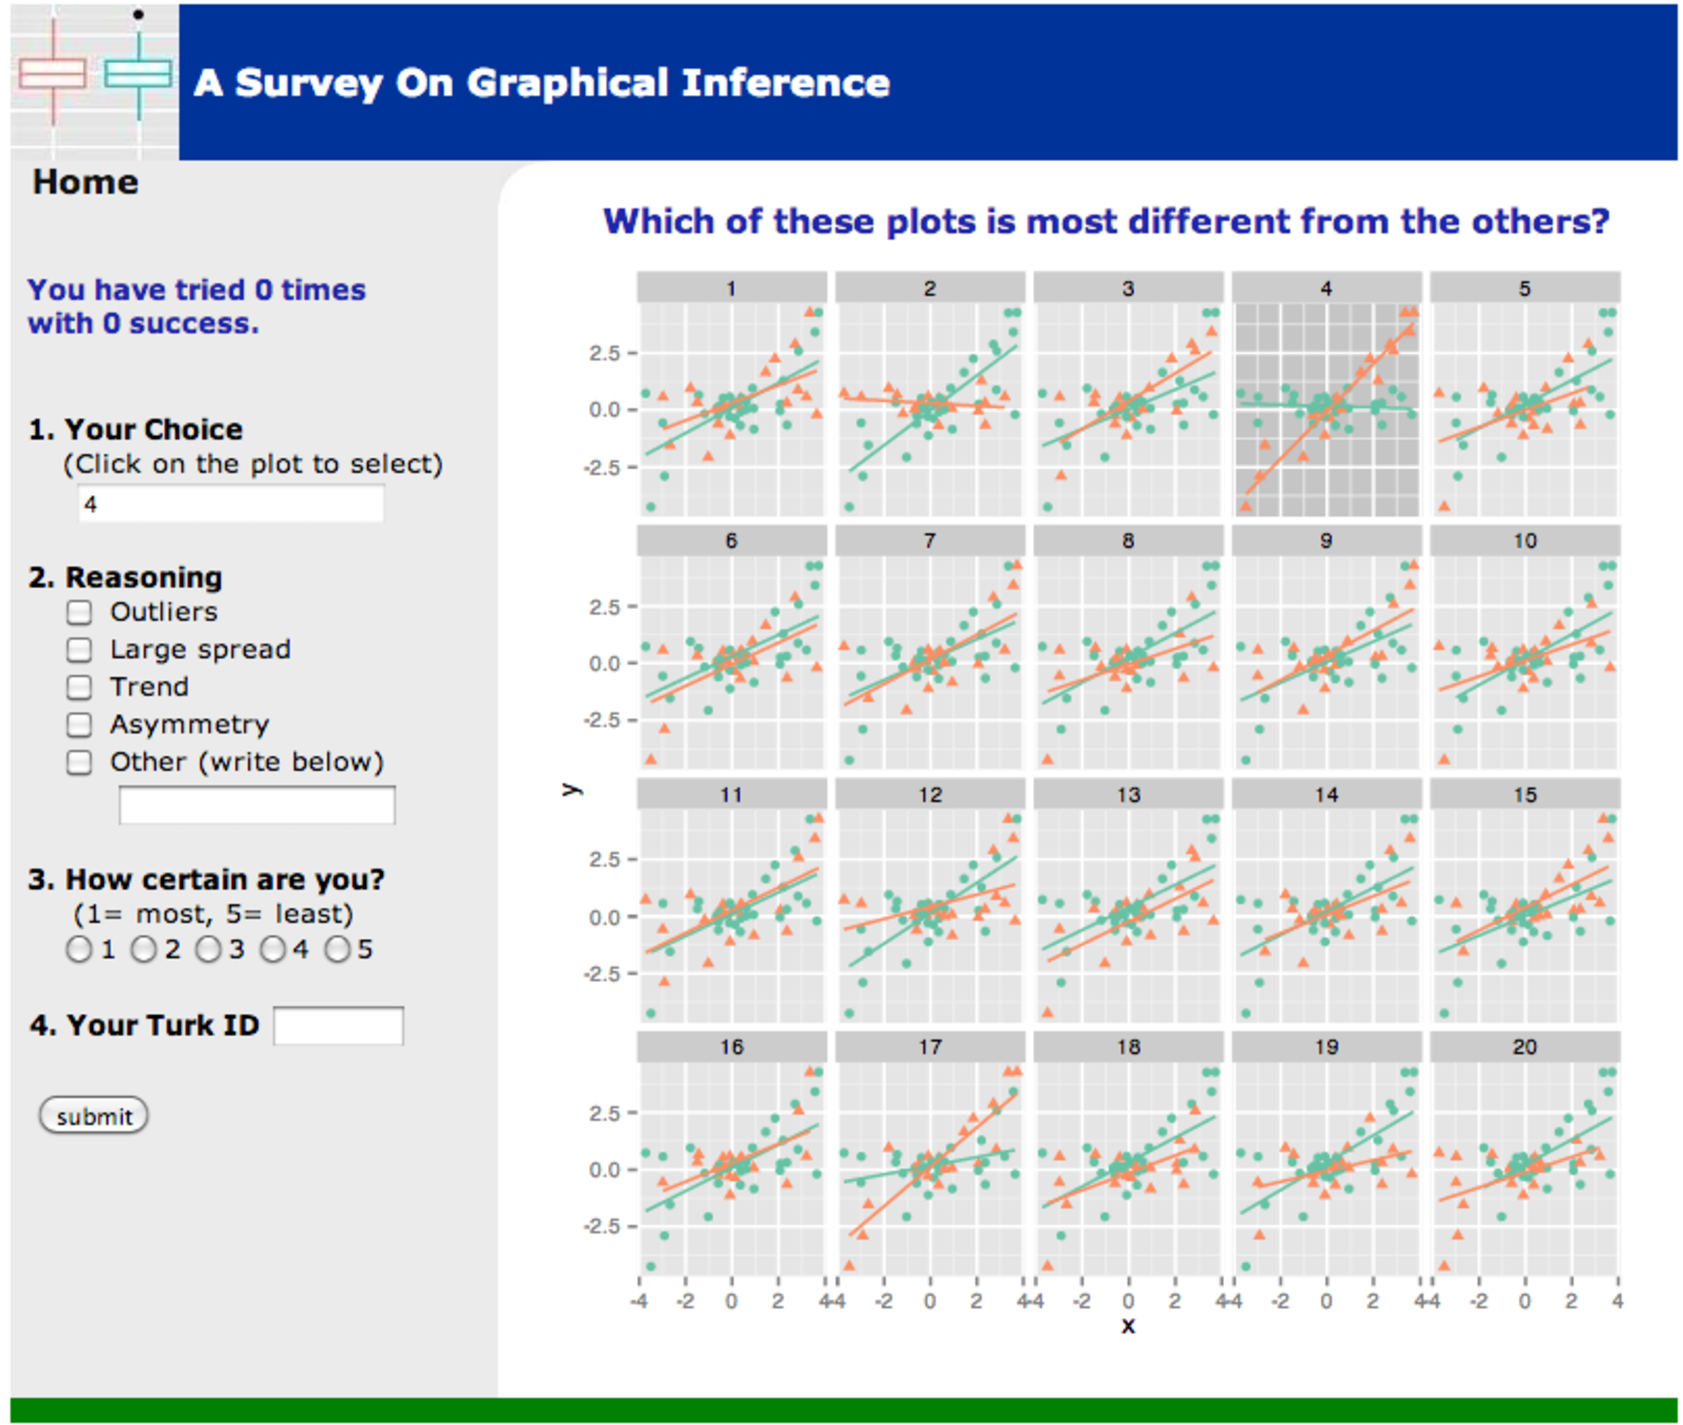
\includegraphics{turk_web.pdf}}
       \caption{A sample data collection form. Lineups are presented at random for evaluations by the turk workers. Scalable Vector Graphics (SVG) is used so that observer can click on the lineup to pick certain plot. Once a plot is selected it gets shaded and the number appears in the choice text box.}
       \label{fig:turk_web}
\end{figure}

One of the nice features of the form in Figure \ref{fig:turk_web} is the use of Scalable Vector Graphics (SVG) for lineup which enables an observer to give feedback with the ease of just a mouse click. If the observer changes mind he or she can click the plot again and deselect it. If needed multiple selection of plots can be allowed, order of selection and deselection can be recorded with time taken for each action. Thats what we meant by saying it is complex in design. 

It is possible to let workers see the statistics of their total feedbacks with number of correct evaluations. This feature can be opted out easily if not necessary. The worker has to provide their turk ID and for next evaluation they don't have to type it again. This allows the worker give feedback using only mouse click. Thats what we meant by saying it is simple for turk worker.

Once the data is submitted a feedback can be provided whether their choice was correct or wrong. This feature can also be opted out easily if not needed. The design of the feedback form is shown in Figure \ref{fig:turk_web_feedback}. This form is also used to collect demographic and educational information about the worker. After the required number of evaluations are obtained, a pass code is given as a proof of the completion of the task which is used for payment purpose later.

\begin{figure}[hbtp]
   \centering
       \scalebox{.4}{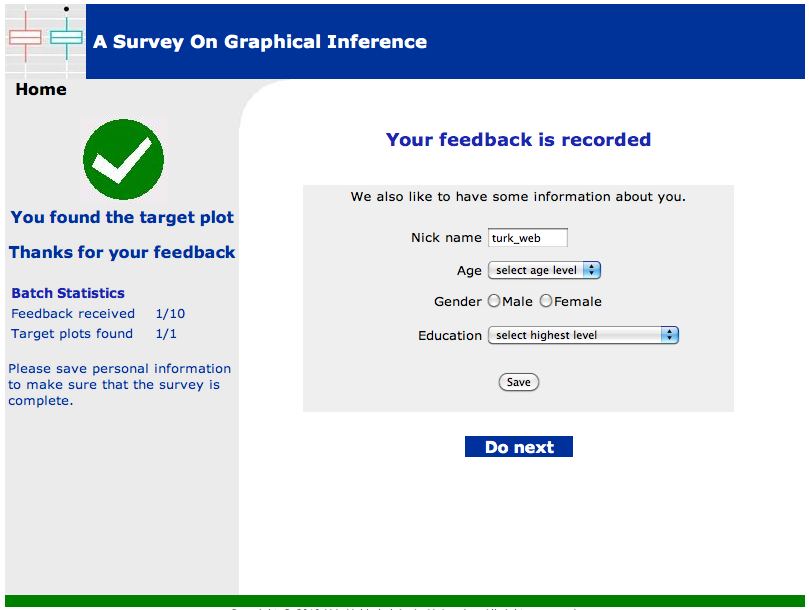
\includegraphics{turk_web_feedback.png}}
       \caption{The turk workers are given feedbacks whether their evaluation for each lineup was correct or not. This works as an incentive for the worker to work more enthusiastically. To ensure the payment, the turk workers have to provide some information using this form.}
       \label{fig:turk_web_feedback}
\end{figure}

Each worker is shown some specific number of lineups for evaluation. These lineups are randomly selected from a pool of lineups designed for evaluations. The algorithm for how the lineups should be selected to show and what would be the order of display is implemented in the form shown in Figure \ref{fig:turk_web}. Also there is a check for invalid or missing information which is implemented using javascript. If users try to go forward without giving any feedback they are not allowed to do that showing a warning message.

%After the evaluation is recorded on a lineup through form shown in Figure \ref{fig:turk_web} another form shown in Figure \ref{fig:turk_web_feedback} is used to give feedback to the turk users whether they correctly identifies the true plot and how many evaluations are recorded from the users. 


\subsection{Database design} The design of the database to store the collected data is shown in Figure \ref{fig:turk_database_design}. It is designed such a way that data from many different experiments can be stored in the same database. In total five separate tables are used. Table turk\_worker contains static information about each turk worker. The location information of each turk worker is stored in ip\_detals table. The information in this table is collected later based on the ip address of each turk worker. Table picture\_delais contains the static information about each lineup. Table feedback is a dynamic table that grows with the number of feedbacks from each turk worker. The multiple activities of the worker are recorded in turk\_activity table. This table also contains the codes provided to the workers once they finish the experiment. For the implementation of the web application we used MySQL database located on a local server.

\begin{figure}[hbtp]
   \centering
       \scalebox{.4}{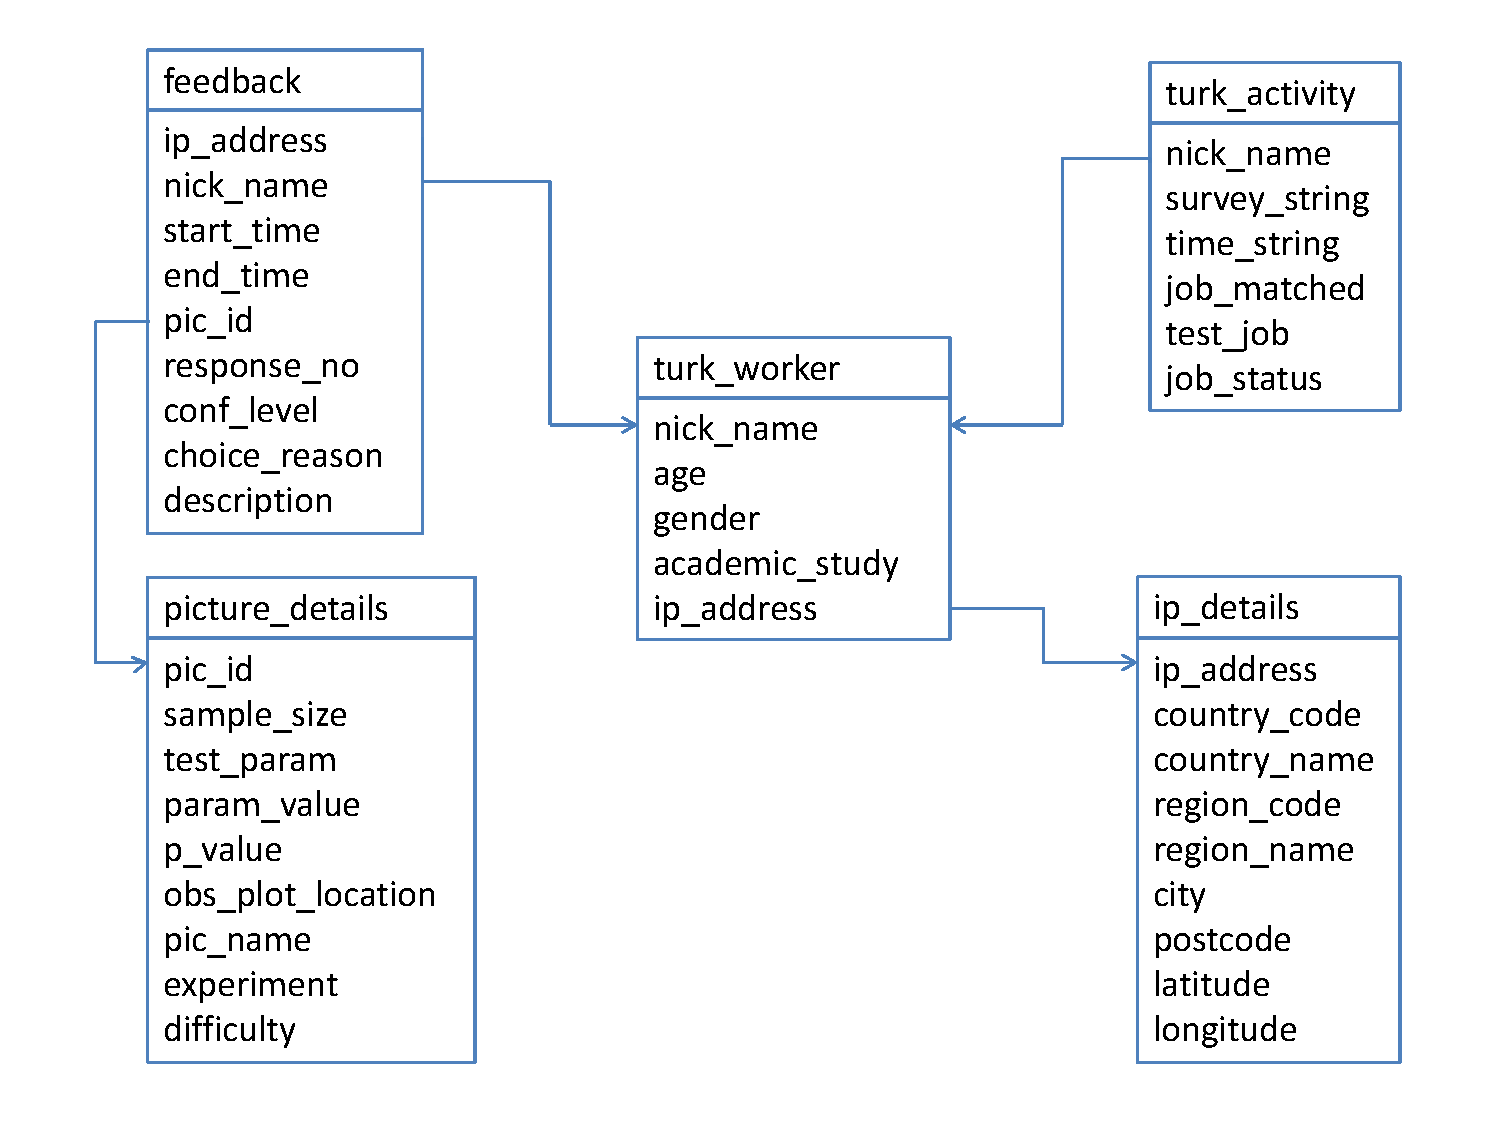
\includegraphics{turk_database_design.pdf}}
       \caption{Relational database design for MTurk experiment data collection. The same database can be used for multiple turk experiments by keeping experiment information in picture\_details table which contains information about the lineups.}
       \label{fig:turk_database_design}
\end{figure}

\subsection{Data collection} 

The homepage of the web displays detailed explanation on how they can perform the task of evaluating the lineups. Several examples with possible answers are provided. It is possible to customize how the workers will proceed from the home page. There are two options; one is to allow them to continue the task where no trial is needed. The second option is to force them to try some lineup before joining the actual experiment. The trial feedbacks are not recorded. As per the requirement of Institutional Review Board (IRB) the workers need to provide the informed consent. For this they have to read and agree with specific IRB approved informed consent. The flow chart for this data collection sequence is shown in Figure \ref{fig:turk_data_flow}.

\begin{figure}[hbtp]
   \centering
       \scalebox{.4}{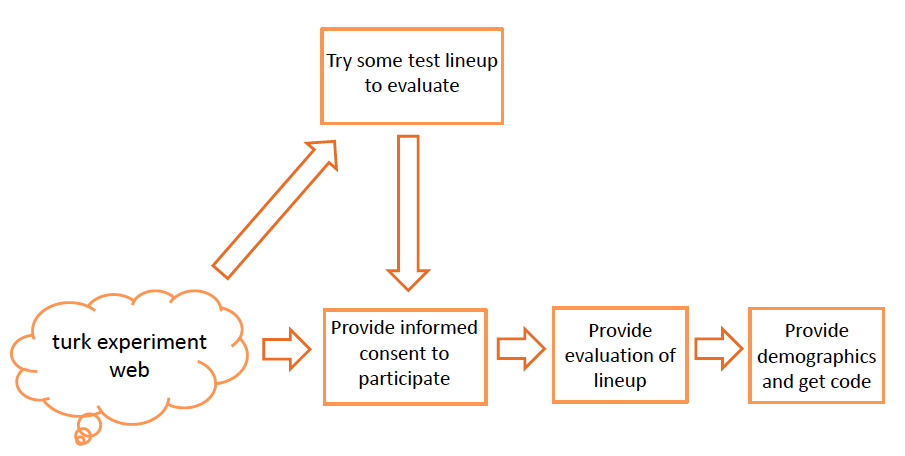
\includegraphics{turk_data_flow.png}}
       \caption{Data collection work flow shows that workers can try some test lineups before going to the live experiment after providing informed consent. This design gives the flexibility to make the trial mandatory, if needed, so that without having enough correct trial evaluations the actual participation can be prevented.}
       \label{fig:turk_data_flow}
\end{figure}


%To collect the survey data we developed a web site that shows a plot to an individual and get feedback from that individual. Each individual is asked to provide feedback for at least 10 different plots. The 10 plots that are shown to an individual are randomly chosen with probability proportional to the number of responses required (the sample size) for that plot.

%The MTurk workers were redirected to the web site and the data were collected, stored automatically into a local database server. Demographic informations such as age group, gender and education levels were also collected. The time taken for each evaluation is computed based on the time the plot was shown and the time the feedback was received. The location of the observer is determined by the ip address of the observer.

%Figure \ref{fig:turk_work_flow} turk workers have to visit the experimental web site and give their consent to participate the survey as per IRB requirement. In the experimental web, there is a option for observers to try some sample lineups to get familiar with the experiment. Once the observers start evaluating the lineups they are sequentially shown a specific number of lineups and at the end they are given a code as a proof for their tusk completion. The payment of the turk worker is processed if they post the code they got from experimental web site. The observers are also asked to provide some demographic information about them to make sure that the code is generated.

The information collected from each individual is shown in Table \ref{tbl:data_info}. Data received from each individual are automatically saved in a secured mysql server maintained by the department of statistics, Iowa state university. 

\begin{table}[hbtp]
\caption{Information Collected from Each Individual}
\centering 
\begin{tabular}{lp{8cm}} 
\hline
Information &  Description \\ %[0.5ex] % inserts table %heading 
\hline
Identification & Nick name or any ID to determine the responses of an Individual \\
Response number & The number of the plot on the lineup plot which the individual thinks the most different than other 19 plots.\\ 
Reason of of choice & Reason why the individual chooses the plot \\
Confidence level & Confidence level of individual choice \\ 
Age group& The age group where the individual belongs \\
Education & The highest level of education completed \\
Gender & Male or female \\
Geographic Location & This information is collected through the ip address of the individual computer \\ 
Time taken & Time taken for each response\\
\hline
\end{tabular}
\label{tbl:data_info}
\end{table}	


%\subsection{Data collection sequence} 


\subsection{Data Security and Validity} 

Some cautious attempts are taken to add security to the data. Server side scripting language PHP is used to connect to database and access or save data. For transferring data from one form to another PHP session variables are used. Cookies are avoided carefully so that no important informations are saved in the cookies. 

To prevent missing information and invalid input JavaScripts are used. For controlling some flow of the work such as showing various messages, JavaScripts are used as well. Careful consideration are made so that no important informations are stored in the java variable or function that could easily be revealed.


\section{Managing Turk Task}\label{sec:turk_task}  

Turk workers are usually small payee workers. There several issues related to the payment of their effort. These are briefly discussed in the following section and we intend to work more on this as we progress through this dissertation work. 

\subsection{Creating Task for Lineup Evaluation} Task description, number of people to recruit, time allowed to finish the task, specify the qualification needed, setting the duration of the task, offering the pay per task.

\subsection{Accepting or Rejecting the Task} In our design we keep a test lineup plot which is very easy to evaluate. The general criteria may be to reject payment when workers do not get that easy test lineup plot. Our experience suggest that there are workers who did not get that test plot but their overall success rate is very high. So depending on only one criteria the payment should not be made. These issues would be addressed in our future work based on the several turk experiments that we intend to carry out.

\subsection{Processing Payment}Amazon Mechanical Turk suggest that each worker gets \$6/hour as wage. Thus we need to estimate how much time a tusk may take to complete and based on that we have to specify the payment for each task. Our experience indicates that a better payment lures more serious workers who usually provide cleaner data which is more reliable. We may study this issue while we do multiple turk experiments.

\subsection{Managing Worker} pay bonus, appreciate worker by sending email, block worker etc.

\section{Turk Data Quality} \label{sec:turk_data}

In this section we intend to analyze the performance of the experiments we did using Amazon Mechanical turk. We have feed back data for the similar plots from both turk workers as well as from the people who regularly participates in the graphics group meeting of our department. We consider later participants as more knowledgeable and trained in seeing pattern in statistical plots. We can use these data to evaluate the performance of the general participants from around the world.



\begin{table}[hbtp]
\caption{Amazon mechanical turk experiments and their properties. Duration in hours per 100 tasks show the popularity of some tasks compared to others.}
\centering
\scalebox{0.9}{
\begin{tabular}{rlrrrrrrr}
  \hline
& Experiment& \multicolumn{2}{c}{ Total Task}& Average & \multicolumn{2}{c}{Duration (hour)} & Payment & Pay rate\\
\cline{3-4} \cline{6-7}
Serial & description & submitted & rejected & time(min) & Actual & 100 task& \$/task & \$/hour\\ 
  \hline
1 & Boxplot & 406 & 106 & 10.68 & 146.48 & 36.08 & 0.50 & 2.81 \\ 
  2 & Scatterplot & 359 &   9 & 10.80 & 42.68 & 11.89 & 1.00 & 5.58 \\ 
  3 & Contaminated plot & 219 &  19 & 13.53 & 126.17 & 57.61 & 1.00 & 2.22 \\ 
  4 & Polar vs Cartesian & 110 &  10 & 20.65 & 11.65 & 10.59 & 1.00 & 2.91 \\ 
  5 & Hist vs density & 234 &  37 & 17.85 & 41.57 & 17.76 & 1.00 & 3.36 \\ 
  6 & Violin vs boxplot & 417 &  17 & 17.95 & 105.87 & 25.39 & 1.00 & 3.34 \\ 
  7 & Group separation & 106 &   6 & 16.13 & 5.15 & 4.86 & 1.00 & 3.72 \\ 
  8 & Sine Illusion & 101 &   1 & 16.52 & 78.38 & 77.60 & 1.00 & 3.63 \\ 
  9 & Gene expression & 103 &   3 & 12.47 & 11.27 & 10.94 & 0.50 & 2.41 \\ 
  10 & Test normality & 406 &   6 & 22.70 & 74.35 & 18.31 & 1.00 & 2.64 \\ 
   \hline
\end{tabular}
}
\label{tbl:mturk}
\end{table}


\begin{figure}[htbp] 
   \centering
   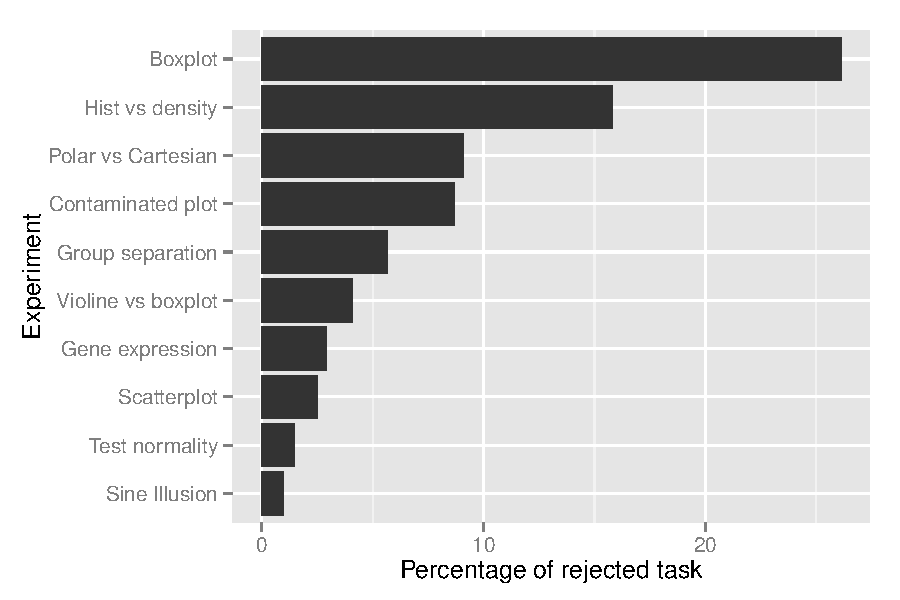
\includegraphics[width=3in]{rejected_task.pdf}
      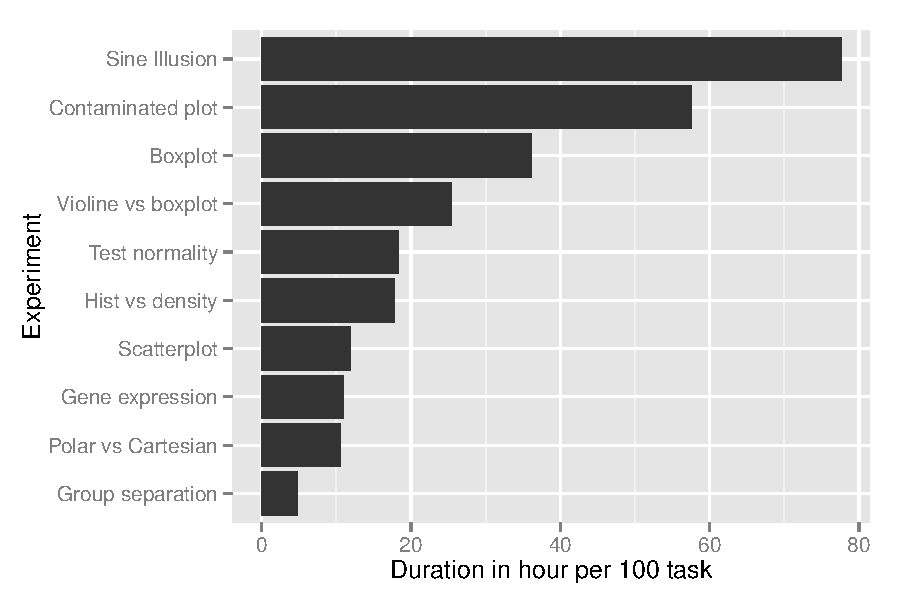
\includegraphics[width=3in]{task_duration.pdf} 
   \caption{Percentage of rejected tasks and duration of each experiment in hour per 100 tasks for each of the 10 experiments. Most of the tasks got rejected for box plot experiment.  Even though the sine illusion experiment took longest to finish the rejection rate is lowest for this experiment.}
   \label{fig:task_duration}
\end{figure}


\subsection{Data Cleaning} Some suggestion about data cleaning based on experimental evidence. What to expect from turk data.

\subsection{Diversity in the Data} Demographics, geographical locations, academic diversity

%\begin{figure}[hbtp]
%   \centering
%       \scalebox{.5}{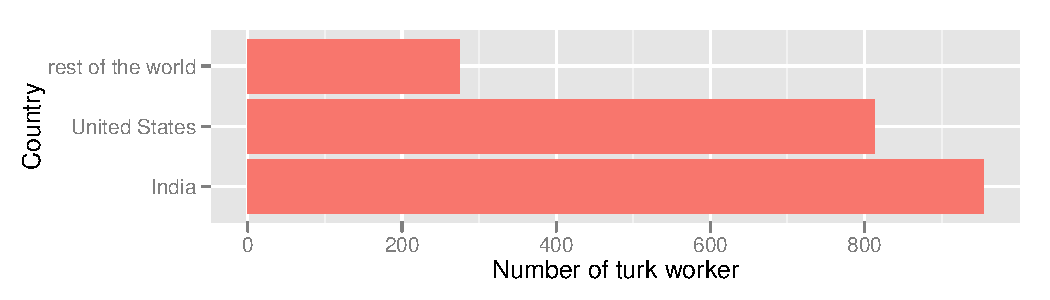
\includegraphics{turker_country.pdf}}
%       \scalebox{.5}{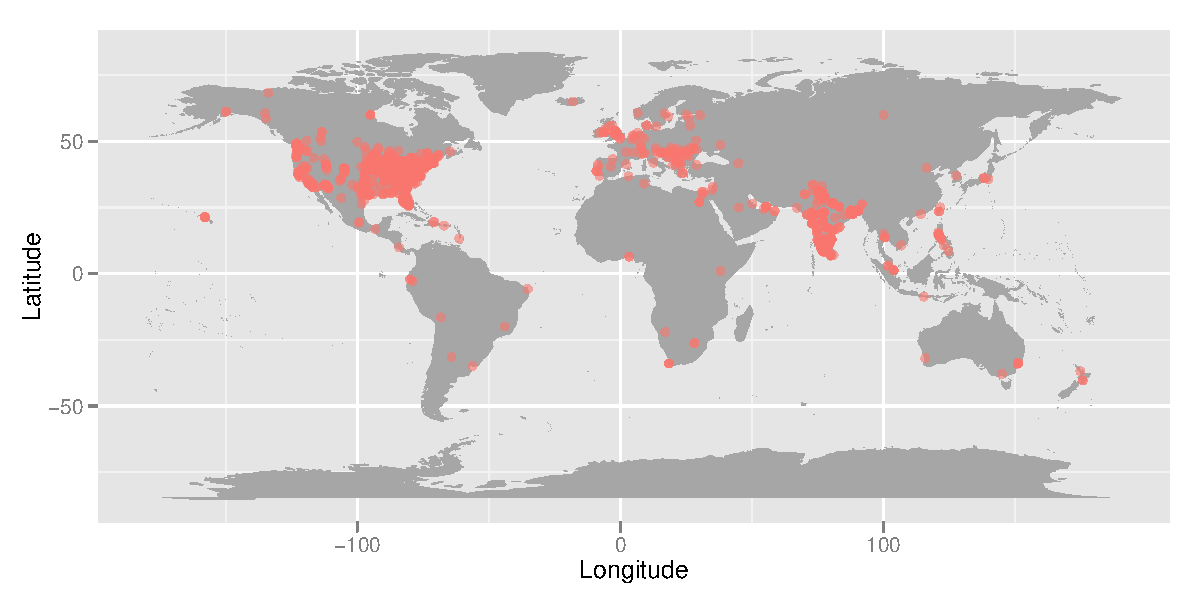
\includegraphics{turker_location.pdf}}       
%       \caption{The location of turk workers on the world map shows the geographical diversity of turk workers even though most of the workers come from India and United States.}
%       \label{fig:rsq}
%\end{figure}

\subsection{Selection Bias} Since data are collected through web interface it is possible to have the selection bias in the turk experiment we did. In this section we intend to analyze to what extent this selection bias has occurred and how we can adjust for this.


Time of the task may recruit from a specific geographical location

Setting up qualification may allow certain workers to do the task

Payment amount may affect the duration of the experiment which may avoid diversity in the geographical locations.


\section{Conclusion} This paper presents a complete solution to the problem of designing a simulation experiment for lineup and recruiting people to get the lineups evaluated. The online application design provides flexibility to control how the multiple lineups would be presented to an observer. Scalable Vector Graphics (SVG) are used for lineup so that observer can click on the lineup to pick certain plot. This also made the multiple plot selection from a lineup easier and convenient. Multiple online experiments are done using this web application and result suggests that the application worked as planned.

One of the main features of the web application is that it produces simple task for the worker who are used to doing so from MTurk but still provides many flexibilities to the researcher who need lineups to be evaluated as per complex experimental requirement. The design of this application allows recruiting people from any source not necessarily just from MTurk. The web application is now hosted on Iowa State University public domain \citep{majumder:turk} and any number of experiments can be done through this web site without changing the core of this application.

The next direction of this work is to make a complete package so that anyone can reproduce this web application, customize according to their need and run the MTurk experiments as part of their research that involves lineups. This would save lot of time which researcher can use focusing on their actual research. This will also help lineup protocol to be used frequently since it will provide an ease of its use in making inferential decisions.

We also intend to set up a web application for public use where researcher can put their lineup for online evaluation. The observer can be recruited from MTurk or any other source including local lab participants. 


%
%\section{Appendix: What do Turk Workers Pick, $R^2$ or $p$-value?} What do people pick in a lineup plot, p-value or $R^2$? To address this issue we obtain the approximate theoretical relationship between $R^2$ and the power of the classical hypothesis test. Suppose we want to test the significance of the slope ( i.e.,  $H_0: \beta=0$ against $\beta \ne 0$) of a continuous covariate $X$ in  a simple linear regression model setting. Also consider $X \sim N(0,1)$. For a sample of size $n$ this gives us 
%\begin{eqnarray*}
%Y_i-\bar{Y}& = & \beta_0+\beta_1X_i+\epsilon_i - \beta_0 - \beta_1 \bar{X}- \bar{\epsilon} \\
%          & = & \beta_1(X_i-\bar{X})+(\epsilon_i-\bar{\epsilon})
%\end{eqnarray*}
%Now 
%\begin{eqnarray*}
%X_i-\bar{X}& = & X_i - \frac1n (X_1 + X_2 + ... + X_i + .....+ X_n) \\
%          & = & X_i - \frac1n X_i - \frac1n \sum_{j \neq i}{X_j}\\
%          & = & (1-\frac1n)X_i - \frac1n \sum_{j \neq i}{X_j}
%\end{eqnarray*}
%
%Thus we have 
%\begin{eqnarray*}
%E(X_i-\bar{X})^2 & = & (1-\frac1n)EX_i^2 - \left( \frac1n \right )^2 (n-1) EX_j^2 \\
%                 & = & (1-\frac1n)^2+ \frac{n-1}{n^2}\\
%                 & = & \frac{n-1}{n}
%\end{eqnarray*}
%
%Similarly we have 
%
%\begin{eqnarray*}
%E(\epsilon_i-\bar{\epsilon})^2 & = & (1-\frac1n)E\epsilon_i^2 - \left( \frac1n \right )^2 (n-1) E\epsilon_j^2 \\
%                 & = & \left((1-\frac1n)^2+ \frac{n-1}{n^2} \right) \sigma^2 \\
%                 & = & \frac{n-1}{n}\sigma^2
%\end{eqnarray*}
%Finally we have expected total sum of square (SST) as
%\begin{eqnarray*}
%E\sum_i{(Y_i-\bar{Y})^2} & = & \sum_i E(Y_i-\bar{Y})^2=\sum_i \left [ \beta_1^2 E(X_i-\bar{X})^2 + E(\epsilon_i-\bar{\epsilon})^2 \right] \\
%                 & = & \sum_i\left[ \beta_1^2 \frac{n-1}{n}+  \sigma^2 \frac{n-1}{n}\right]\\
%                 & = & (n-1)(\sigma^2+\beta_1^2)
%\end{eqnarray*}
%
%We know $E(MSE|X) = \sigma^2$ or $E(SSE/n-2)|X = \sigma^2$ which gives the expected residual or error sum of square as $$E \sum_i (Y_i-\hat Y_i)^2=(n-2)\sigma^2$$
%Thus we have the expected regression sum of squares $SSR =  (n-1)(\sigma^2+\beta_1^2) - (n-2)\sigma^2 = (n-1) \beta_1^2+\sigma^2$ This gives $$R^2=\frac{(n-1) \beta_1^2+\sigma^2}{ (n-1)(\sigma^2+\beta_1^2)}$$
%
%
%\begin{figure}[hbtp]
%   \centering
%       \scalebox{.3}{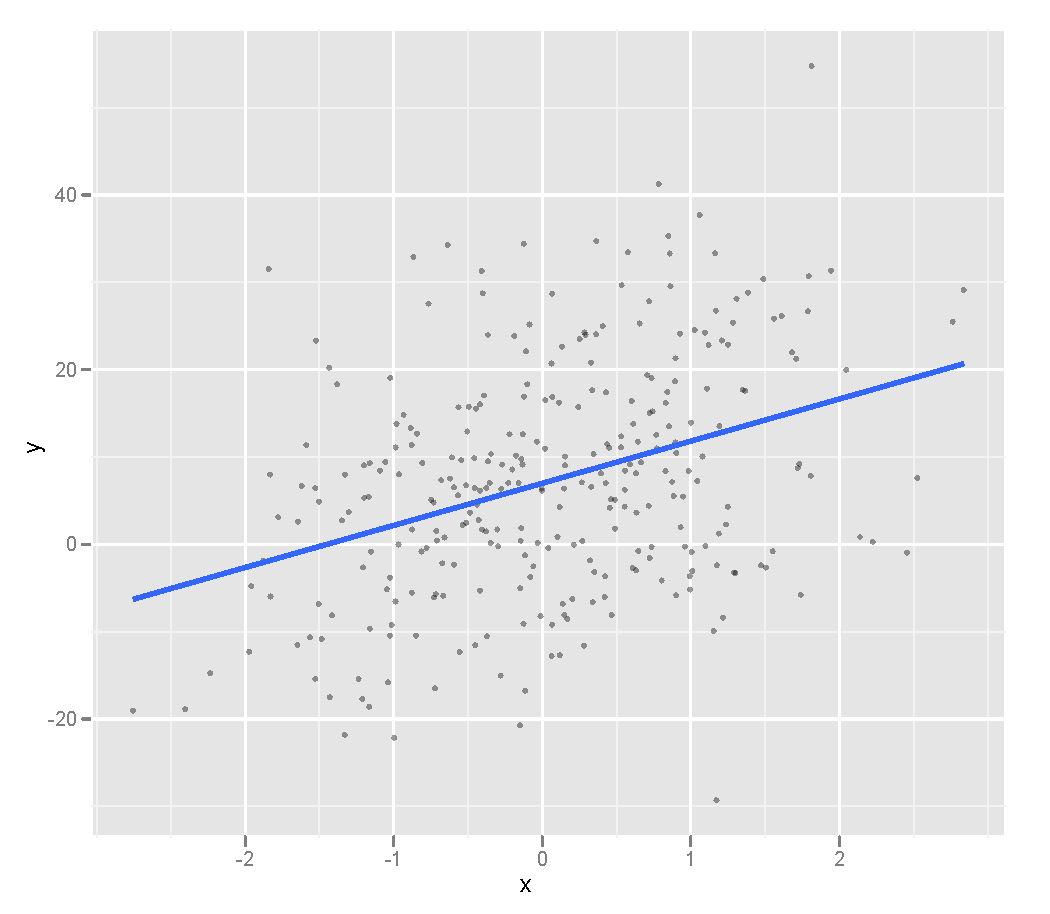
\includegraphics{scatter_plot_beta_4.pdf}}
%       \caption{Scatter plot of data generated for $\beta_0$=6, $\beta_1$=4, sample size $n =300$ and $\sigma = 12$. $R^2$ for this data was obtained as 0.1309 showing that the model could not successfully explain the variation in $Y$. But notice in figure \ref{fig:power_rsq} that power for $\beta$=4 is almost 1. So, Can we conclude that $R^2$ does not have any effect in deciding whether $H_0: \beta_1=0$ should be rejected or not?}
%       \label{fig:plot_beta_4}
%\end{figure}
%
%
%\begin{figure}[hbtp]
%   \centering
%       \scalebox{.35}{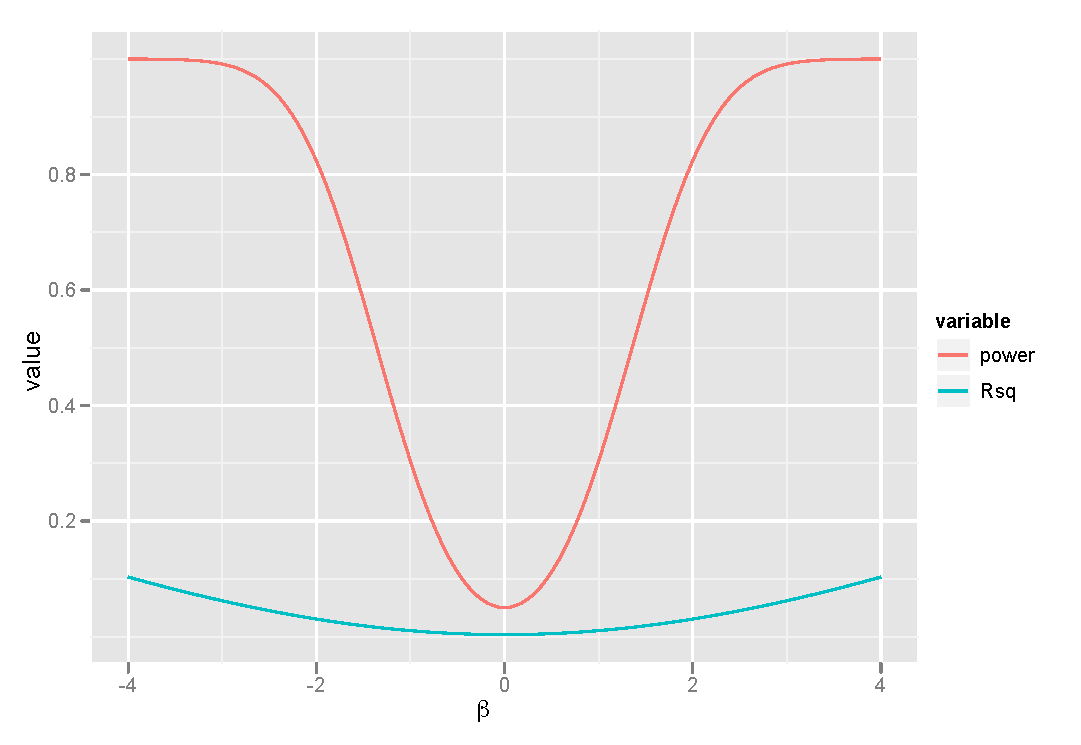
\includegraphics{power_300_12.pdf}}
%       \caption{Power curve and $R^2$ values for sample size $n =300$ and $\sigma = 12$. Notice that for a small value of $R^2$ (0.1) the power is almost 1.}
%       \label{fig:power_rsq}
%\end{figure}
%
%
%\begin{figure}[hbtp]
%   \centering
%       \scalebox{.35}{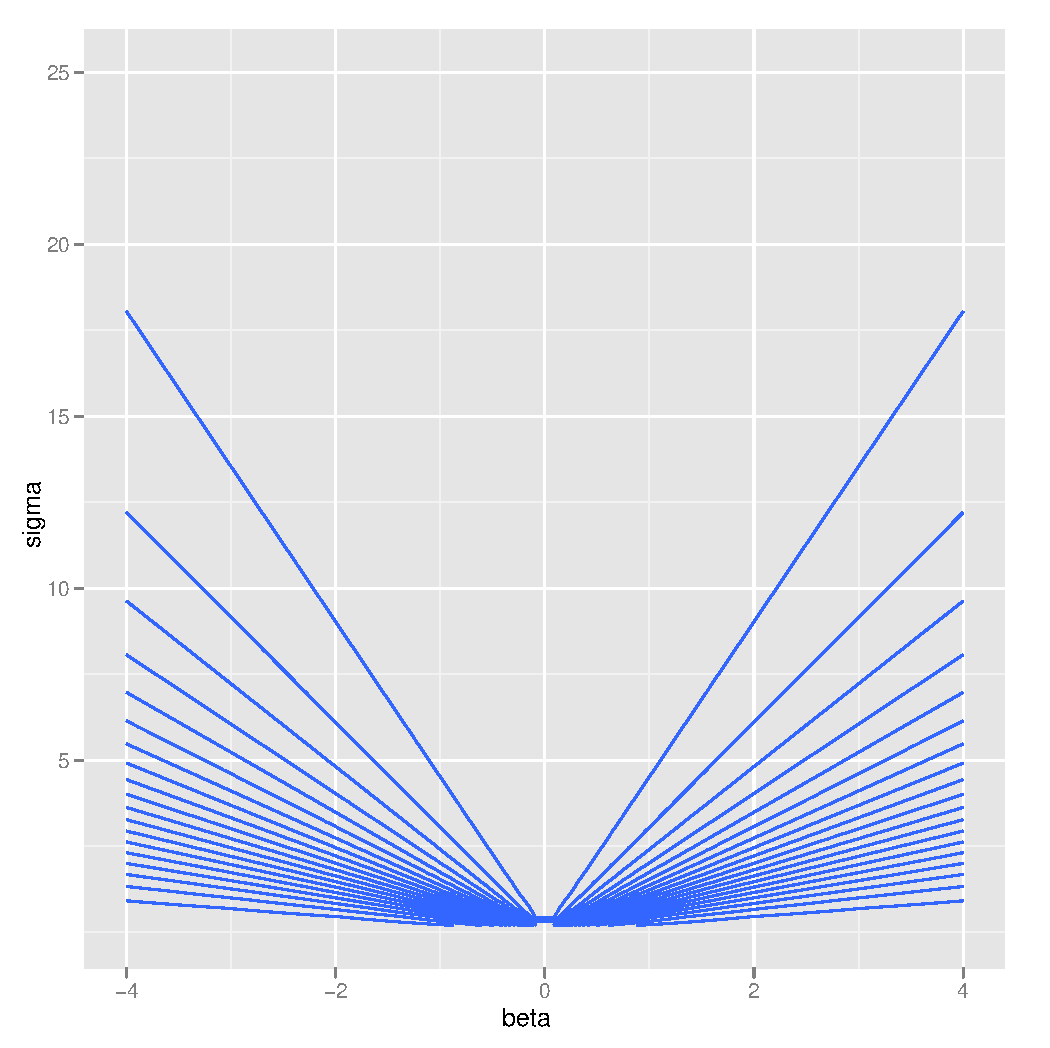
\includegraphics{rsquare_contour.pdf}}
%       \scalebox{.35}{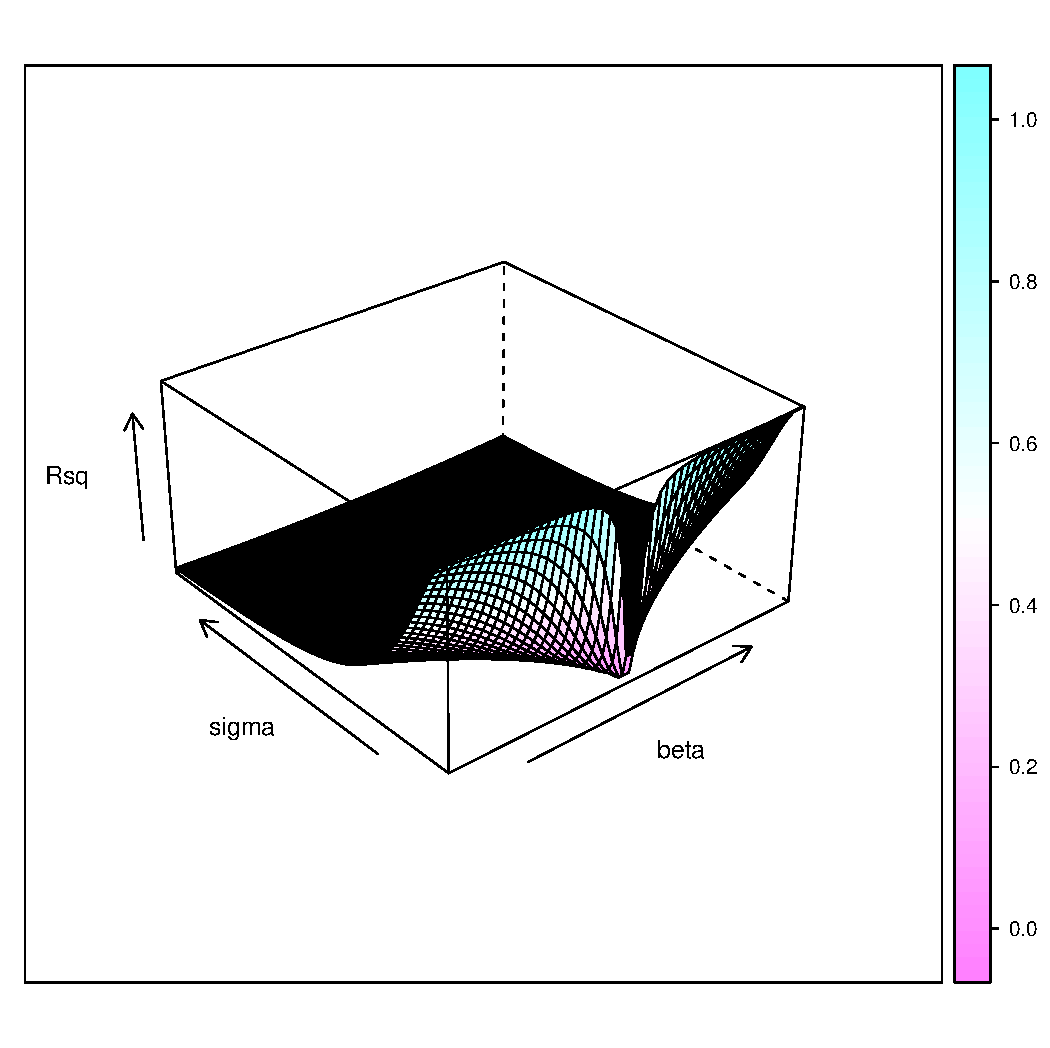
\includegraphics{rsquare_beta_sigma.pdf}}
%       \caption{Contour and surface plots of $R^2$ for sample size $n =300$. The values for $R^2$ goes down sharply with $\sigma$ and $\beta$.}
%       \label{fig:contour_rsq}
%\end{figure}
%
%\begin{figure}[hbtp]
%   \centering
%       \scalebox{.35}{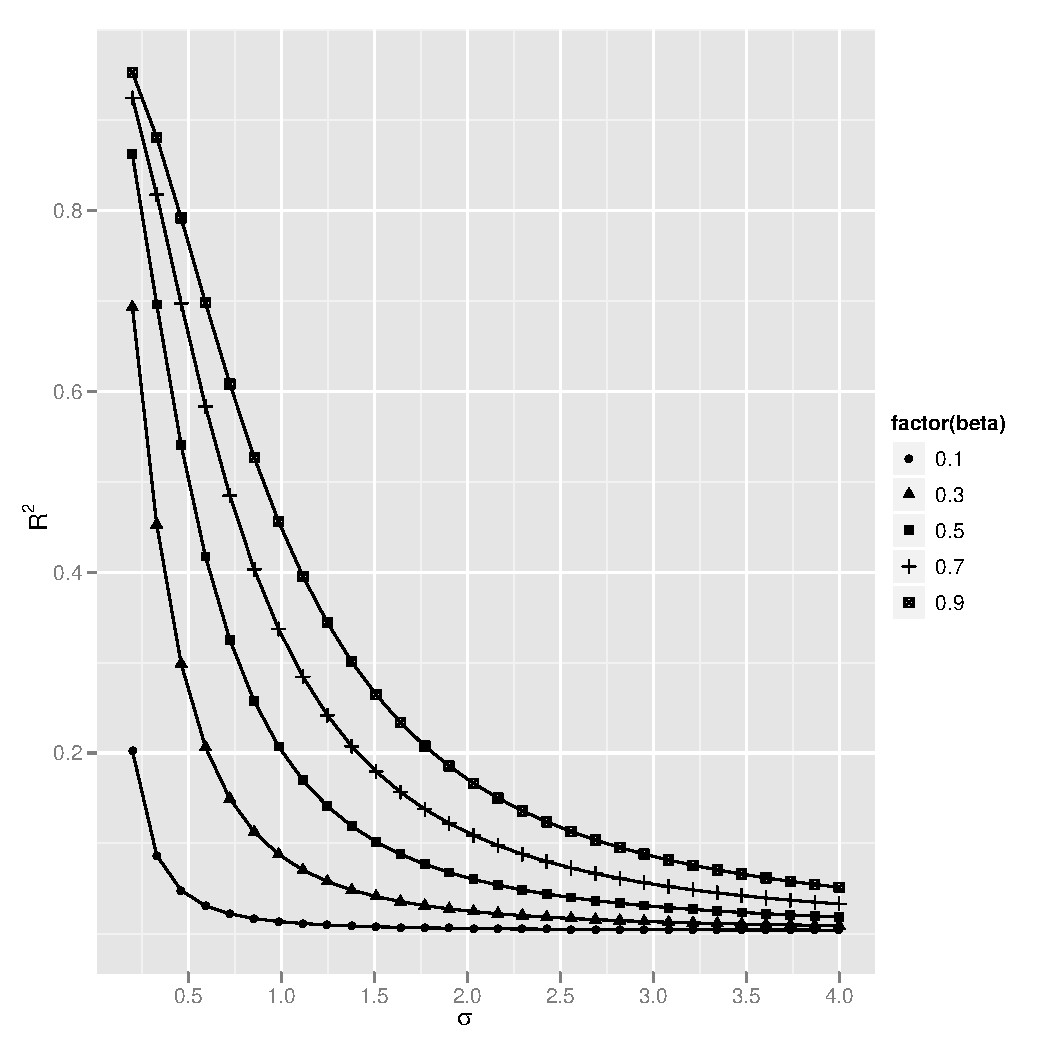
\includegraphics{rsquare_beta_sigma_lines.pdf}}
%       \scalebox{.35}{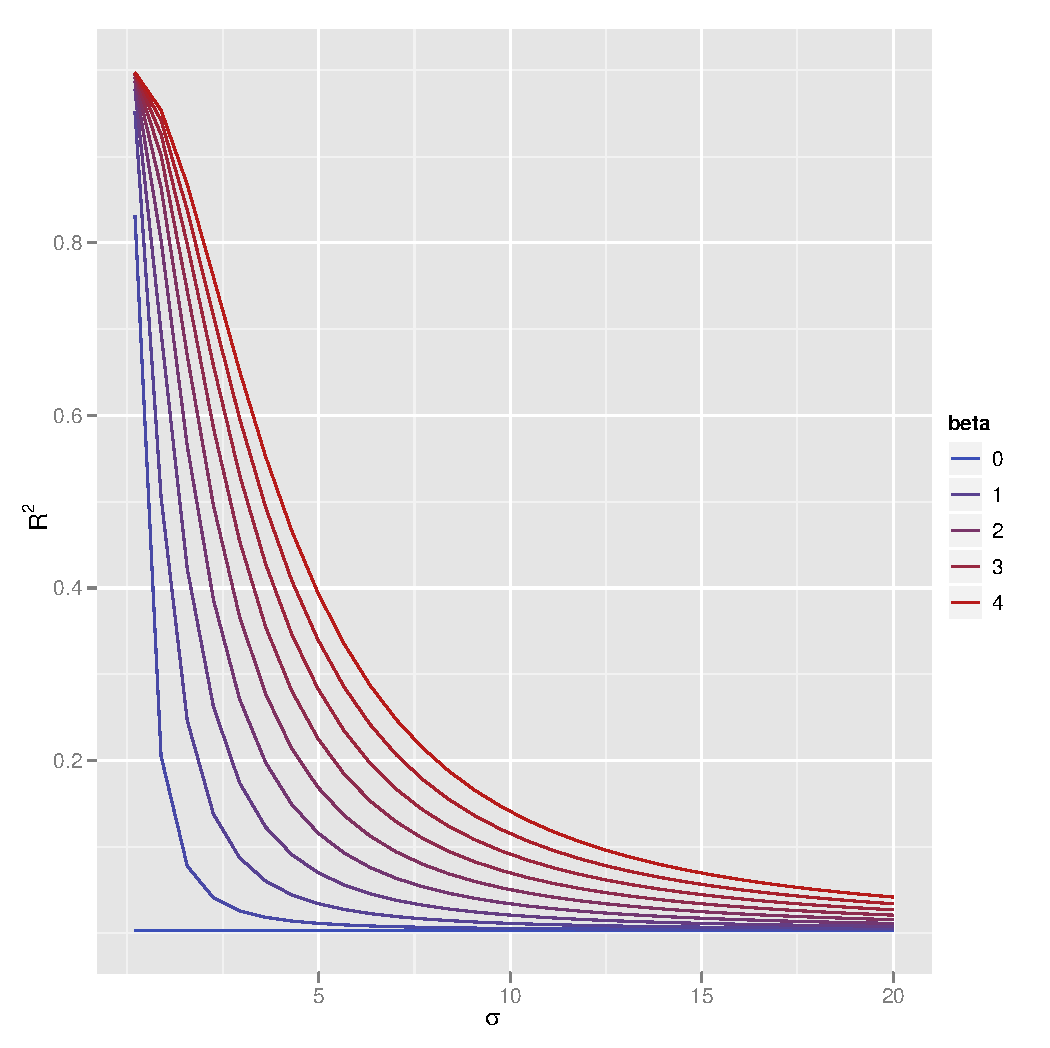
\includegraphics{rsquare_beta_sigma_lines1.pdf}}       
%       \caption{Relationship of $R^2$ with $\sigma$ and $\beta$ for sample size $n =300$. The values for $R^2$ goes down sharply with $\sigma$ and $\beta$.}
%       \label{fig:rsq}
%\end{figure}
%



%\bibliographystyle{plain}
\bibliographystyle{asa}
\bibliography{references} 


\end{document}


